\documentclass[lineno]{jfm}

\usepackage{graphicx}
%\usepackage{epstopdf,epsfig}
\usepackage{newtxtext}
\usepackage{newtxmath}
\usepackage{natbib}
\usepackage{hyperref}
\usepackage{mathtools}
\usepackage{commath}
\usepackage{todonotes}




\hypersetup{
    colorlinks = true,
    urlcolor   = blue,
    citecolor  = black,
}
\newtheorem{lemma}{Lemma}
\newtheorem{corollary}{Corollary}
\newcommand{\RomanNumeralCaps}[1]
\linenumbers


% Bryan's Marcros
\renewcommand{\aa}{\mathbf{a}}
\newcommand{\bd}{\partial}
\newcommand{\DD}{\mathcal{D}}
\newcommand{\eeta}{\boldsymbol{\eta}}
\newcommand{\FF}{\mathbf{F}}
\newcommand{\GG}{\mathbf{G}}
\newcommand{\nnu}{\boldsymbol{\nu}}
\newcommand{\ssigma}{\boldsymbol{\sigma}}
\newcommand{\rr}{\mathbf{r}}
\newcommand{\RR}{\mathbf{R}}
\renewcommand{\SS}{\mathbf{S}}
\newcommand{\xx}{\mathbf{x}}
\newcommand{\uu}{\mathbf{u}}
\renewcommand{\vv}{\mathbf{v}}
\newcommand{\yy}{\mathbf{y}}
\newcommand{\pderiv}[2]{\frac{\partial #1}{\partial #2}}


% {\MakeUppercase{\romannumeral #1}}

%\title{Two-Dimensional Vesicles Under External Flow via Integral Equation Method}
\title{Modeling Two-Dimensional Vesicle Hydrodynamics with Hydrophobic Attraction Potential Simulations}
%\author{Alan N. Jones\aff{1}
%  \corresp{\email{JFMEditorial@cambridge.org}},
%  H.-C. Smith\aff{1}
% \and J.Q. Long\aff{2}}
%
%\affiliation{\aff{1}STM Journals, Cambridge University Press, The Printing House, Shaftesbury Road, Cambridge CB2 8BS, UK
%\aff{2}DAMTP, Centre for Mathematical Sciences, Wilberforce Road, Cambridge CB3 0WA, UK}


\author{
Szu-Pei Fu\aff{1},
Bryan Quaife\aff{2},
Rolf Ryham\aff{1}, \and
Yuan-Nan Young\aff{3}
}
 \affiliation{
\aff{1}Department of Mathematics, \\Fordham University, Bronx, New York 10458, USA
\aff{2}Department of Scientific Computing, \\Florida State University, Tallahassee, Florida 32306, USA
\aff{3}Department of Mathematical Sciences, New Jersey Institute of Technology,\\ Newark, New Jersey 07102, USA
 }





\begin{document}
\maketitle

\begin{abstract}
In this work, we study the dynamics of many-body systems immersed in a viscous fluid with a specified interparticle force. In particular, we apply a hydrophobic attraction potential (HAP) using a Janus type granular system to model lipid bilayer membranes. Coupling with an efficient integral equation method for rigid bodies in Stokes flow and an previous developed HAP solver, the deformations of a two-dimensional vesicle such as tank-treading motion and membrane ruptures can be observed under different values of the shear rate. Moreover, an efficient integral equation method is adopted for solving the screened Laplace equation and the mobility problem where it can accurately calculate hydrophobic and hydrodynamic interactions between near touched boundaries.
\end{abstract}


\begin{keywords}
Authors should not enter keywords on the manuscript, as these must be chosen by the author during the online submission process and will then be added during the typesetting process (see \href{https://www.cambridge.org/core/journals/journal-of-fluid-mechanics/information/list-of-keywords}{Keyword PDF} for the full list).  Other classifications will be added at the same time.
\end{keywords}

{\bf MSC Codes }  {\it(Optional)} Please enter your MSC Codes here



\section{\label{intro}Introduction}
Described by de Gennes as ``another animal in soft matter physics", the Janus particle (often a spherical particle with a hydrophobic and a hydrophilic hemisphere) exhibits complex aggregate, clustering and self-assembly into meso- and macroscopic structures that are relevant to a wide range of applications in biology and bioengineering. Whether it is surface chemistry or polarity under an external field, the dynamics of Janus particles is inevitably the combination of long-range hydrodynamics interactions in the presence of short- and intermediate-range particle-particle interactions. 

Recently Fu {\it et al.} illustrated that the hydrophobic interactions between Janus particles in a viscous solvent can be used as a coarse-grained model to capture the mechanics of an elastic bilayer membrane of amphiphilic macromolecules such as lipids \cite{Fu2020_SIAM}. Depending on the total number of Janus particles and their geometry, in a viscous solvent, Janus particles are found to aggregate to form a micelle, a patch of bilayer membrane with open ends, and a self-enclosed bilayer membrane (a vesicle). Using a hybrid continuum model for the interactions between amphiphilic particles in a viscous solvent and formulating it in a boundary integral formulation, Fu {\it et al.} showed that the membrane granularity during fusion and fission of bilayers can be accurately captured. 
%This boundary integral formulation has inspired more recent work

In molecular dynamics (MD) simulations, the lipid bilayer membranes are often approximated by an implicit solvent coarse-grained model for lipids (as in the Martini code), where their hydrodynamic interactions are simplified by an implicit solvent. The long-range hydrodynamic interactions and the induced long-range lipid interactions can be captured by combining the Dry Martini with a lattice Boltzmann MD \cite{Brandner2019_SciRep}. Brandner {\it et al.} used this methodology to simulate the hydrodynamics of a nano-sized vesicle under a shear flow, and reproduced the well-know vesicle hydrodynamics  such as tank-treading, tumbling and inter-leaflet slippage (reported from simulations of the Helfrich-type continuum model). 

In this work we extend the hybrid continuum model in \cite{Fu2020_SIAM} for the Janus suspension to incorporate the collective hydrodynamics of a Janus suspension under various flows: a linear shear flow, an elongation flow, and a Poiseuille flow. We demonstrate that a vesicle made of Janus particles does behave like a vesicle in these flowing conditions. Furthermore we also show that the hybrid continuum model allows us to investigate the inter-leaflet slippage and rupture of a bilayer membrane due to an imposed flow. 

This paper is organized as follows. In \S~\ref{sec:governing_eqs} we present the formulation for the Janus particles in a viscous fluid in the zero-Reynolds number regime. In \S~\ref{sec:IEM} we extend the hybrid continuum model for a Janus suspension to include the effects of a far-field flow via the mobility problem formulation. In \S~\ref{validation} we present validation of our model, and in \S~\ref{results} we present simulation results for a vesicle of Janus bilayer membrane under various flowing conditions. Finally we provide discussion and outlook for future directions in \S~\ref{conclusion}.







\section{Governing  Equations\label{sec:governing_eqs}}
\subsection{\label{mobility}Mobility Problem}
We consider a suspension of $N_b$ particles suspended in a
two-dimensional unbounded domain. The boundary of each particle is
denoted by $\Gamma_i$ so that $\bd \Omega = \Gamma_1 \cup \Gamma_2 \cup
\cdots \cup \Gamma_{N_b}$. Assuming the flow is Stokesian, the governing
equations are
\begin{alignat}{3}
  -\mu \Delta \uu + \nabla p &= \mathbf{0}, 
    && \xx \in \Omega, \\
  \nabla\cdot \uu &= 0, \qquad && \xx \in \Omega, \\
  \uu - \uu_\infty &\to \mathbf{0}, && |\xx| \to \infty,
\end{alignat}
%
where $\uu$ is the velocity, $\mu$ is viscosity, $p$ is the pressure,
and $\uu_\infty$ is the background flow. Since each particle $\Gamma_i$
with center $\aa_i$ is a rigid body, its velocity satisfies 
\begin{align}
  \vv(\xx) = \vv_i + \omega_i (\xx - \aa_i)^\perp, \quad 
    \xx \in \Gamma_i,
\end{align}
where $\vv_i$ is its translational velocity and $\omega_i$ is its
angular velocity. Here, $\langle x, y \rangle^{\perp} = \langle -y, x
\rangle$. Therefore, the no-slip boundary condition on each particle is
\begin{align}
  \uu(\xx) = \vv_i + \omega_i (\xx - \aa_i)^\perp, \quad
    \xx \in \Gamma_i.
\end{align}
To determine the translational and angular velocities of each particle,
we assume some imposed forces $\FF_i$ and torques $T_i$ acting on each
particle. Since the small particles are intertialess, force balance
gives 
\begin{alignat}{2}
  \label{eqn:force}
  \FF_i &+ \int_{\Gamma_i} \ssigma \cdot \nnu_i \, ds = \mathbf{0},
  && i=1,\ldots,N_b,\\
  \label{eqn:torque}
  T_i &+ \int_{\Gamma_i} (\xx - \aa_i)^\perp \cdot 
    (\ssigma \cdot \nnu_i) \, ds = 0, \qquad && i=1,\ldots,N_b,
\end{alignat}
where $\ssigma = -p \mathbf{I} + \mu \left(\nabla \uu + \nabla \uu^T
\right)$ is the hydrodynamic stress tensor (pressure tensor). The
process of finding the translational and angular velocities given a
force and torque is referred to as the mobility problem.


\subsection{Imposed Forces}
The imposed forces and torques contain two parts. The first part comes
from the hydrophobic attraction potential (HAP). This potential was
introduced in~\cite{Fu20} and models hydrophobic attraction by solving
the screened Laplace equation boundary value problem
\begin{alignat}{2}
  \label{SL}
-\rho^2 \Delta u + u &=0,            && \xx \in \Omega,\\
\label{SLbc}
u(\xx) &= f_i(\xx),\qquad  && \xx \in \Gamma_i, \\
\label{SLff}
u &\to 0,                          &&|\xx| \to \infty,
\end{alignat}
where $f_i$ is a material label with $f_i = 0$ ($1$) representing
hydrophilic (hydrophobic) portions of the surface, and $\rho$ is the
decay length of attraction. The forces and torques for this attraction
are 
\begin{align}
  \label{eqn:hydrophobicAttraction}
  \FF_i^{\text{hydro}} = \int_{\Gamma_i} {\bf T}\cdot \nnu_i \, dS, 
    \quad 
  T_i^{\text{hydro}} = \int_{\Gamma_i} (\xx - \aa_i)^{\perp} \cdot ({\bf T} \cdot \nnu_i) dS,
\end{align}
where
\begin{align}
  \label{eq:stress}
\mathbf{T}
= \gamma\rho^{-1}u^2 \mathbf{I} + 2\rho\gamma \left(\tfrac{1}{2}|\nabla
  u|^2 \mathbf{I} - \nabla u\otimes \nabla u\right)
\end{align}
is the hydrophobic stress tensor. The parameter $\gamma$ is interfacial
tension. The forces $\FF_i^{\text{hydro}}$ and torques
$T_i^{\text{hydro}}$ are responsible for forming particle aggregates
that partially sequester the hydrophobic portions of the particle
surface.

The second part of the imposed forces and torques comes from repulsion
between proximal particles. Given a pair particles indexed with $i$ and
$j$, we find the two points $\tilde{\xx}_i \in \Gamma_i$ and
$\tilde{\xx}_j \in \Gamma_j$ that are closest to one another. We then
define the repulsion force and torque
\begin{align}
%  \label{eqn:REPUL}
%  \FF_i^{\text{repul}} = \sum_{i=1}^{N_b} \frac{\xx_{ij} -
%  \yy_{ij}}{\rho_{ij}} P(\rho_{ij}),\quad 
%  T_i^{\text{repul}} = \sum_{i=1}^{N_b} (\xx_{ij} - \aa_i)^{\perp}\cdot
%  \frac{\xx_{ij} - \yy_{ij}}{\rho_{ij}} P(\rho_{ij})
%  \\
%
  \label{eqn:REPULforce}
  \FF_i^{\text{repul}} &= \sum_{j \neq i} 
    \frac{\tilde{\xx}_i - \tilde{\xx}_j}
    {|\tilde{\xx}_i - \tilde{\xx}_j|} 
    P'(|\tilde{\xx}_i - \tilde{\xx}_j|), \\
  \label{eqn:REPULtorque}
  T_i^{\text{repul}} &= \sum_{j \neq i} 
    (\tilde{\xx}_i - \aa_i)^{\perp} \cdot 
    \frac{\tilde{\xx}_i - \tilde{\xx}_j}
    {|\tilde{\xx}_i - \tilde{\xx}_j|} 
    P'(|\tilde{\xx}_i - \tilde{\xx}_j|).
\end{align}
The repulsion profile $P(r)$ is zero for distances $r$ larger than a
repulsion length scale $\rho_0$. As such,~\eqref{eqn:REPULforce}
and~\eqref{eqn:REPULtorque} ignore particles $\Gamma_j$ outside a
tubular neighborhood of $\Gamma_i$. For $0 \leq r < \rho_0,$ we use
$P(r) = M(1 - \sin(r/\rho_0))$ where $M$ is sufficiently large to
prevent particle collisions. Then, the total imposed force and torque
are
\begin{align}
  \FF_i = \FF_i^{\text{hydro}} + \FF_i^{\text{repul}},\quad
  T_i = T_i^{\text{hydro}} + T_i^{\text{repul}}, \qquad
  i=1,\ldots,N_b.
\end{align}


\subsection{Time Marching}
By solving the mobility problem, we obtain translational and angular
velocities of the $N_b$-body system. A second-order Adams-Bashforth
scheme updates the particle positions and orientations. By including the
repulsion force~\eqref{eqn:REPULforce} and
torque~\eqref{eqn:REPULtorque}, particle collisions are avoided even
when using a relatively large time step. 



%This paper is organized as follows. Chapter 2 introduces the mobility problem..... The integral equation method for solving $N_b$-body system with details of .... are included in Chapter 3. We provide numerical results of vesicle simulations in Chapter 4. Finally, we conclude the work and briefly give the picture of our future work.



%%%
\section{Integral Equation Method}
\label{sec:IEM}
Computing the hydrophobic attraction potential and the particle forces
and torques requires solving an elliptic partial differential equation
(PDE) in an unbounded complex domain. We recast both these PDEs as
boundary integral equations (BIEs). We discretize each BIE at $N$ points
on each of the $N_b$ particles with a collocation method. Integrals that
are smooth are computed with the spectrally-accurate quadrature rule,
and nearly-singular integrals, caused by close contact between two
particles, are computed with a high-order interpolation-based quadrature
rule~\cite{qua-bir2014}. After discretizing and applying quadrature, the
resulting linear system is solved with matrix-free GMRES, and we
guarantee that the number of GMRES iterations is mesh-independent by
using second-kind BIEs.


\subsection{HAP Boundary Integral Equation}
Similar to our previous work~\cite{Fu20}, we represent the HAP as a
double-layer potential
\begin{align}
  \label{eqn:HAP_DLP}
  u(\xx) = \frac{1}{2\pi} \int_{\bd\Omega} \pderiv{}{\nnu_\yy}
    K_0 \left(\frac{|\xx - \yy|}{\rho}\right) \sigma(\yy) \, ds_\yy,
    \quad \xx \in \Omega,
\end{align}
where $K_0$ is the zeroth-order modified Bessel function of the first
kind. By requiring that the density function $\sigma$ satisfies the
second-kind integral equation
\begin{align}
  f(\xx) = \frac{1}{2}\sigma(\xx) + 
    \frac{1}{2\pi}\int_{\bd\Omega} \pderiv{}{\nnu_\yy}
    K_0 \left(\frac{|\xx - \yy|}{\rho}\right) \sigma(\yy) \, ds_\yy,
    \quad \xx \in \bd\Omega,
\end{align}
the HAP double-layer potential~\eqref{eqn:HAP_DLP} satisfies the
screened Laplace equation~\eqref{SL}--\eqref{SLff}. To calculate the
hydrophobic force and torque, the gradient of the double-layer
potential~\eqref{eqn:HAP_DLP} must be computed on the boundary of each
particle. In Appendix~\ref{sec:appendixA}, we show that the force and
torque calculations can be expressed in terms of integral that are
non-singular.

\subsection{Mobility Problem Boundary Integral Equation}
Following previous work of~\cite{Lukas19}, we represent the velocity as
the sum of a double-layer potential and the $N_b$ Stokeslets and Rotlets
\begin{align}
  \label{eqn:velocity}
  \uu(\xx) = \uu_\infty(\xx) + \DD[\eeta](\xx) + 
    \sum_{i=1}^{N_b} \left(\SS(\xx,\aa_i) \FF_i + 
    \RR(\xx,\aa_i) T_i\right), \quad \xx \in \Omega.
\end{align}
The double-layer potential is
\begin{align}
  \DD[\eeta](\xx) = \frac{1}{\pi} \int_{\bd\Omega} 
    \frac{\rr \cdot \nnu}{\rho^2} \frac{\rr \otimes \rr}{\rho^2}
    \eeta(\yy) \, ds_\yy,
\end{align}
where $\rr = \xx - \yy$ and $\rho = |\rr|$. The Stokeslet and Rotlet
centered at $\aa_i$ are
\begin{align}
  \SS(\xx,\aa_i)\FF_i &= \frac{1}{4\pi} \left(-\log(\rho) + 
    \frac{\rr \otimes \rr}{\rho^2} \FF_i \right), \\
  \RR(\xx,\aa_i)T_i &= \frac{1}{4\pi} \frac{\rr^\perp}{\rho^2} T_i,
\end{align}
where $\rr = \xx - \aa_i$ and $\rho = |\rr|$. The Stokeslet is
torque-free and has force $\FF_i$ while the Rotlet force-free and has
torque $T_i$. Therefore, the velocity~\eqref{eqn:velocity} satisfies the
total force~\eqref{eqn:force} and torque~\eqref{eqn:torque} conditions
if the double-layer potential $\DD[\eeta]$ is force- and torque-free.
Matching the limit of~\eqref{eqn:velocity} with the rigid body motion,
and imposing that $\DD[\eeta]$ is force- and torque-free, the density
function $\eeta$, translational velocity $\vv_i$, and angular velocity
$\omega_i$ satisfy
\begin{alignat}{3}
  \nonumber
  \vv_i + \omega_i (\xx - \aa_i)^\perp &= \uu_\infty(\xx)
    -\frac{1}{2} \eeta(\xx) + \DD[\eeta](\xx) \\
  \label{eqn:SKIE}
    + \sum_{j=1}^{N_b} &
    \left(\SS(\xx,\aa_j) \FF_j + \RR(\xx,\aa_j) T_j\right),
    \quad &&\xx \in \bd \Gamma_i,\: i=1,\ldots,N_b, \\
  \label{eqn:mobility1}
  \int_{\bd\Gamma_i} \eeta \cdot \nnu_i \, ds &= {\bf 0}, 
  &&i = 1,\ldots,N_b, \\
  \label{eqn:mobility2}
  \int_{\bd\Gamma_i} \eeta\times(\xx-\aa_i)^\perp \cdot \nnu ds &= 0,
  &&i = 1,\ldots,N_b.
\end{alignat}

The trapezoid rule is used to approximate each of the integrals in
equations~\eqref{eqn:mobility1} and~\eqref{eqn:mobility2}, and the
double-layer potential equation~\eqref{eqn:SKIE} is approximated with
either the trapezoid rule, or the interpolation-based near-singular
integration quadrature rule. After discretizing and applying appropriate
quadrature rules, the result is a $(2NN_b + 3N_b) \times (2NN_b + 3N_b)$
linear system that we precondition with a block-diagonal preconditioner.
We note that other BIE formulations of the mobility problem use
single-layer potentials~\cite{cor-gre-rac-vee2017, rac-gre2016} or both
single- and double-layer potentials~\cite{cor-vee2018}.



%%%


\section{\label{validation}Model Validation}

\subsection{Jeffery Orbit}


The preliminary test of the proposed model using the integral equation method is the numerical validation in Jeffery orbits of single ellipsoidal particle under a shear flow $\dot x = \dot\gamma y$ where $\dot\gamma$ is the shear rate. An ellipsoidal particle is initially placed with its center of mass fixed at the origin and the angle between the major axis and the $y$-axis is denoted as $\Theta = 0^\circ$. Based on the theoretical Jeffery orbits with respect to the target angle $\Theta(t)$, 

\begin{equation}
\Theta(t) = \tan^{-1}\left(\frac{a}{b}\tan \left(\frac{ab \dot\gamma t}{a^2+b^2}\right)\right),
\end{equation}
%
where $a$, $b$ are semi-major and semi-minor axes, and the test aspect ratios of the particle are $2$ and $3$. Figure~\ref{figure1} shows that the proposed integral equation method has a perfect agreement with the theoretical result from the Jeffery orbits.


\begin{figure}
\centering
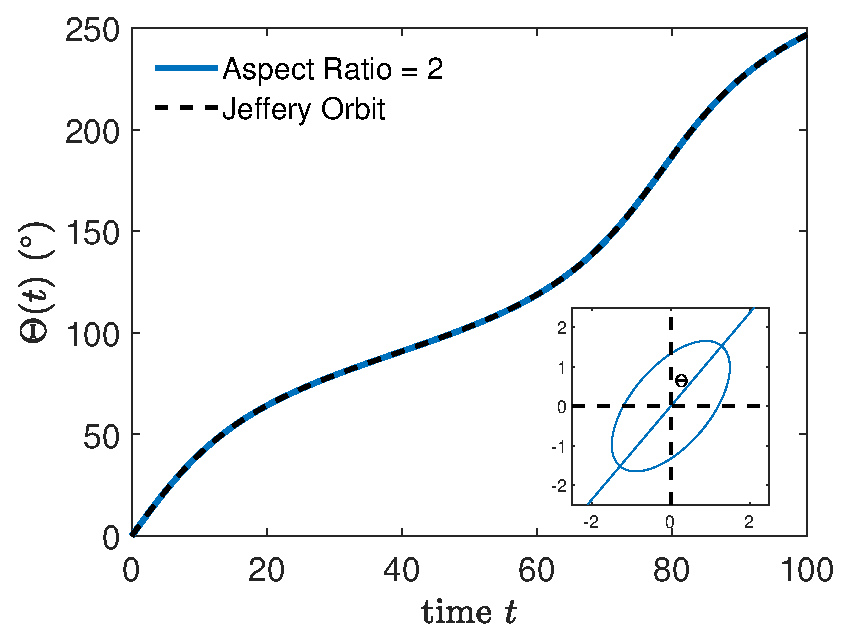
\includegraphics[width=0.4\textwidth]{JefferyOrbit2.eps}
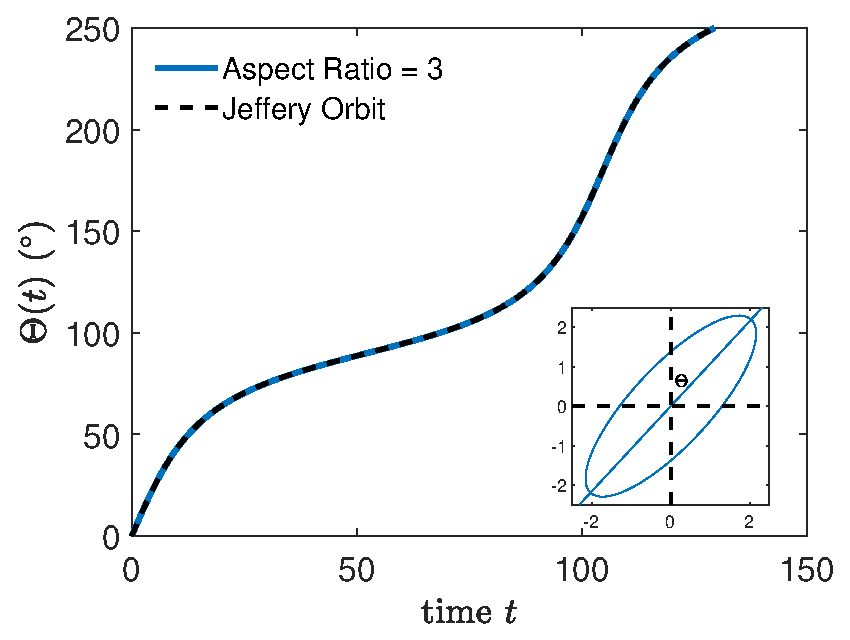
\includegraphics[width=0.4\textwidth]{JefferyOrbit3.eps}
  \caption{Comparisons of the target angle $\Theta(t)$ versus time $t$ between the theoretical Jeffery orbit with $\dot\gamma=0.1$ and the result from the integral equation method. The schematic of the simulation setup is shown in the inset of the figure. Here two cases of aspect ratio are validated, $a/b = 2$ and $a/b=3$.
  }
    \label{figure1}
\end{figure}

\subsection{Self-Assembly and Relaxtion}

In order to examine the dynamics of the Janus-vesicle using the HAP coupling with hydrodynamics interactions, for the target bilayer, a circular initial shape is chosen to perform the relaxation run. 
This vesicle-like structure consists of $N=58$ disks with particle radius $r=0.5$ and the starting diameter of 
the vesicle is about $8.5$ length units.
The starting center of mass position of the Janus-vesicle is pinned at the origin and particle velocities are tracked to determine the initial configuration for later use such as single and multiple vesicle simulations. 
This will prevent some numerical instability issues when the minimum of the total energy is not achieved. 
For instance, the dynamics of the bilayer under a shear flow may reach different outcomes.
Figure~\ref{figure2}(a) shows that the magnitudes of mean velocity components ${\bf v}=\{v_x,v_y\}$ decrease exponentially with an approximation decaying rate $\sim0.005$. In the same figure, the variation of the mean particle orientation $\theta$ also decreases over a period of time as expected from the self-assembly property of the model. This implies that a local energy minimum and the equilibrium configuration are 
nearly attained. 
The time step size $\Delta t=0.2$ is used for all simulations in this work including the relaxation run.
Figure~\ref{figure2}(b) shows the configuration difference between starting and ending frames in the relaxation run. The Figure~\ref{figure2}(c)-(d) demonstrate the fluid pressure profile of two configurations. The pressure inside the permeable Janus-vesicle decreases as expected.

\begin{figure}
\centering
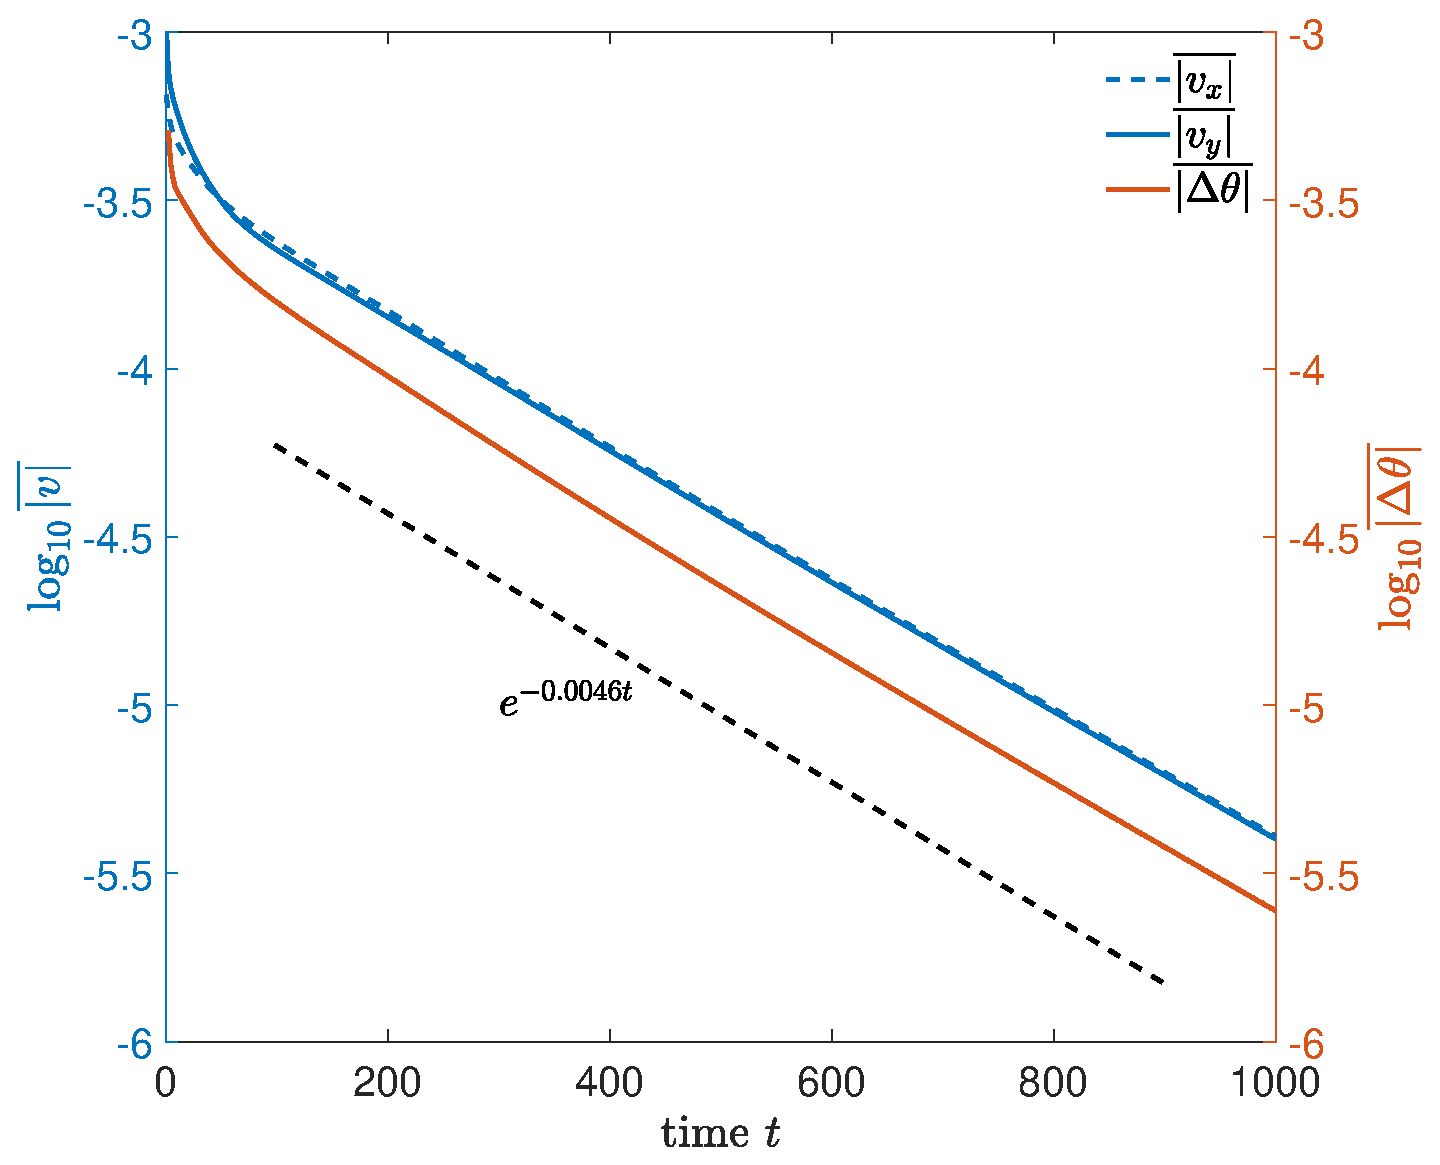
\includegraphics[height=2in]{relax.eps}
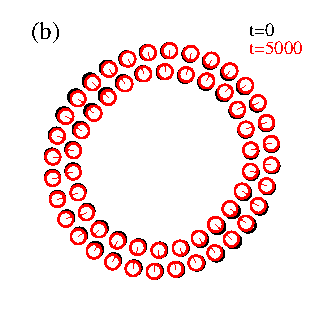
\includegraphics[height=2in]{relax2.eps}\\
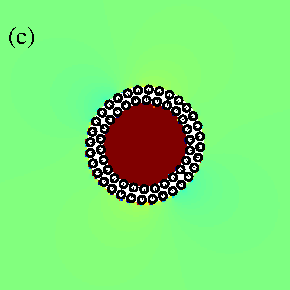
\includegraphics[height=2.in]{N58_0pres.pdf}
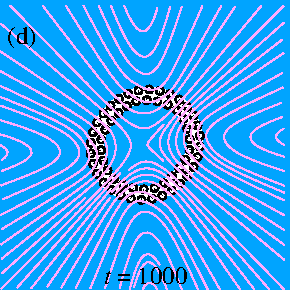
\includegraphics[height=2.in]{N58_5000pres.pdf}
%  \todo[inline]{Put pressure of each of the two configurations below
%  this.}
  \caption{Vesicle relaxes under a quiescent flow. (a) The blue dashed and solid curves are mean magnitudes of the particle velocities in $x$ and $y$ directions, respectively. The red curve shows the decreasing trend of the mean magnitude of particle orientation change. The black dashed line shows the reference of how all magnitudes decay. (b) Bilayer configurations for $t=0$(gray) and $t=1000$(red) with particle directors.
  (c)-(d) show the fluid pressure profiles for $t=0$ and $t=1000$ where the background curves indicate the streamlines. In panel (c), the pressure value in internal fluid is much higher than the pressure outside of the bilayer. After the relaxation, this immersed permeable bilayer approaches a steady state as shown in panel (d).
  }
    \label{figure2}
\end{figure}




%%%


\section{\label{results}Numerical Results}

\todo[inline]{Introduce dimensionless shear rate here (and check the numbers)}

Following the relaxation experiments of the Janus-vesicle, this section will focus on the behavior of vesicles 
under a number of flow types. To extract physical quantities of the target structure using the proposed model, the scaling laws and the dimensionless units are given as follows.
The length unit is scaled by the length of phospholipids $l=2.5$ nm and the force is scaled from the 
interfacial tension $\gamma=4.1$ pN nm$^{-1}$ from ~\cite{Ryham16}. We then be able to calculate the corresponding 
time scale $\tau = 0.38$ ns. With the same framework, \cite{Fu20} provides the bending rigidity 
$\kappa=8.51$ kT.

For the $N$-body Janus-vesicle, we denote a constant initial radius $R_0=\sqrt{A_0/4\pi}$ with initial area $A_0$ and the dimensionless shear rate $\chi$ is referred from~\cite{Finken08} and~\cite{Shaqfeh11},
\begin{align}
  \chi = \dot\gamma \frac{\mu R_0^2}{\kappa},
\end{align}
%
where $\dot\gamma$ the dimensional shear rate, and $\mu$ the fluid viscosity.


\subsection{Tank-Treading Vesicles}

\subsubsection{Vesicle in a Shear Flow}

To study the deformation of a closed bilayer structure under a shear flow using the proposed algorithm, 
we adopt a widely tested numerical simulation in both continuum and molecular dynamics models, single vesicle under a shear flow. The well known results indicate that the vesicle does tank-treading when there is no viscosity contrast in both inside and outside of the structure.
Given a set of various shear rates, with no viscosity difference between internal and external fluids, 
the vesicle-like granular structure is initially placed in a quiescent flow for obtaining an equilibrium shape.


The snapshots of the simulation for single vesicle in a shear flow are shown in Figure~\ref{figure3}.
Panel (a) shows the initial circular shape obtained from the relaxation run and the deformed 
configuration of the vesicle after a period of time ($t=4000$) is in panel (c). The color presented in the figure 
is the strength of the action due to the hydrophobic attraction. From weak to strong action field, the color
varies from blue to red.
To demonstrate the tank-treading behavior of the vesicle, panels (b) and (d) provide the streamlines of the 
fluid velocity over the whole computational domain when the shear flow passes through the structure. The tank-treading motion of the structure is then observed, for instance, the particle velocities in panel (d) indicate a clockwise tank-treading movement.


\begin{figure}
\centering
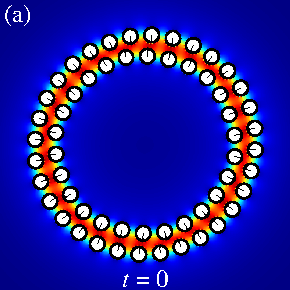
\includegraphics[width=0.3\textwidth]{N58_0.pdf}
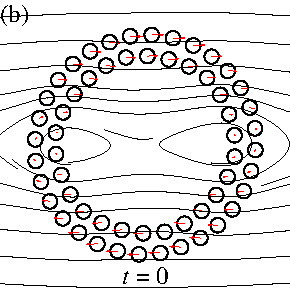
\includegraphics[width=0.3\textwidth]{N58_vel_0.pdf}\\
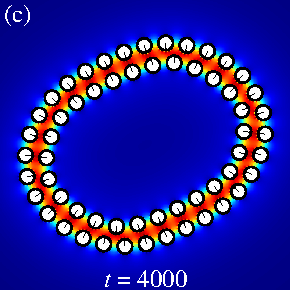
\includegraphics[width=0.3\textwidth]{N58_20000.pdf}
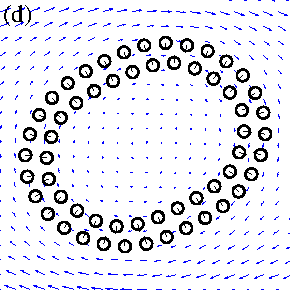
\includegraphics[width=0.3\textwidth]{N58_vel_20000.pdf}
  \caption{Vesicle under a shear flow where the shear rate $\dot\gamma=0.0025$: 
  (a) Initial configuration of 58-body vesicle; 
  (b) The fluid velocity plot with respect to the configuration in (a); Streamlines are plotted in the background
  as solid curves. Red arrows represent the particle velocities.
  (c) Deformed vesicle after $20000$ steps. The tank-treading motion occurs after reaching the state shown in panel (c).
  (d) The fluid velocity plot with respect to the configuration in (c);
  The background colors in panels (a) and (c) represent the strength of the hydrophobic attraction potential. The blue region shows no action and the red region with the bilayer gives the strongest action.
  }
    \label{figure3}
\end{figure}
%

In order to extract more physical properties of the proposed model, we track the total length of the bilayer structure, the reduced area over the time, and the excess length. Here the enclosed area and the length of the structure are calculated from the midplane. 
These results are shown in Figure~\ref{figure4} where we compare results from a set of shear rates $\dot\gamma=\{0.002,0.0025,0.003,0.0035\}$. 
The reduced area is given by $A^* = 4\pi A/L^2$ where $A$ is the vesicle area and $L$ is the arc length of the vesicle with respect to the midplane. 
Furthermore, the excess length is given by $\Delta=L/\sqrt{A^*/\pi}-2\pi$.
Since the starting configuration is close to a circular shape, the reduced area decreases from a value very close to $1$. It is clear that a slower shear rate generates a higher reduced area and has a faster convergence. 
With a converging total arc length, a slower shear rate also produces a smaller excess length.
The small oscillations in all results are due to the granularity of the bilayer which tend to having a slightly non-smooth curve in simulations. Overall the total lengths of the bilayer have the same converging value in all test shear rates. Moreover, based on the 
numerical experiments, we observe that the reduce area converges relatively early when the shear rate is lower than $\dot\gamma=0.003$. 

An interesting phenomenon also rises up in the proposed setup where the inter-monolayer slip occurs 
between two leaflets. When a shear rate is large enough, take $\dot\gamma = 0.005$ as an example, 
Figure~\ref{figure5} shows the schematic of the test. A particle pair is initially marked and we then track the positions and mean angle $\theta(t)$ between particle relative position with respect to the vesicle center over the time. It is clear to see that the outer leaflet always has larger 
tangential velocity than the one from inner leaflet and the mean angle $\theta(t)$ increases. 
This inter-leaflet sliding phenomenon is consistent with what has been seen
in articles in molecular dynamics simulations. %%% need some citations

\begin{figure}
\begin{center}
\hspace{-0.6cm}
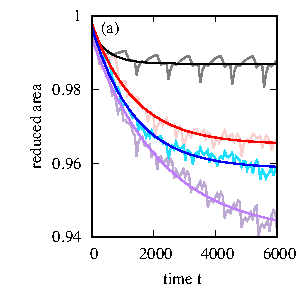
\includegraphics[height=2in]{ReducedArea.pdf}
\hspace{0.6cm}
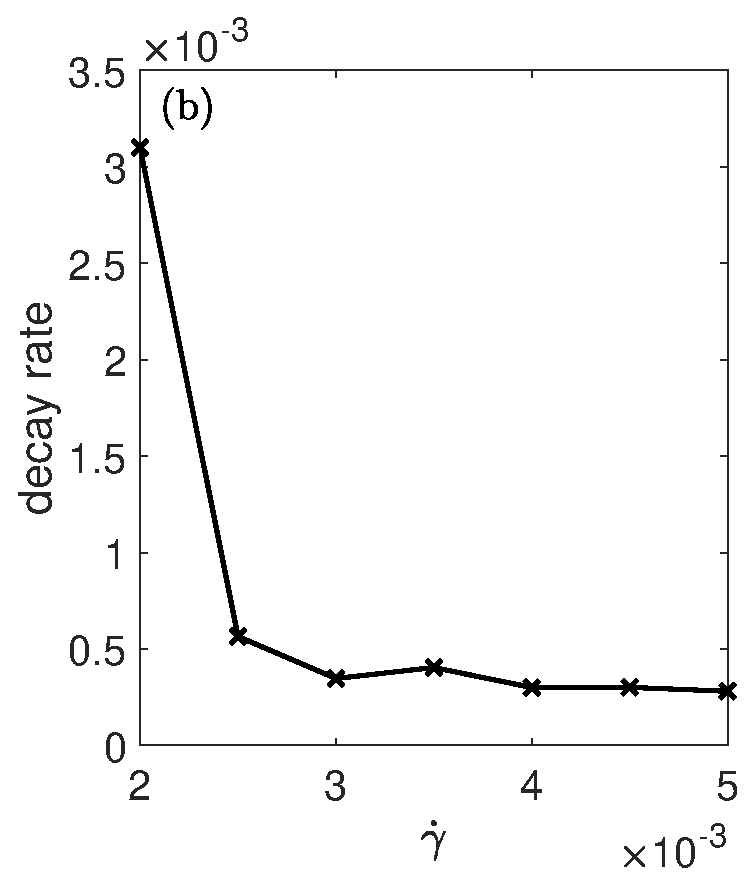
\includegraphics[height=2in]{DecayRate.eps}\\
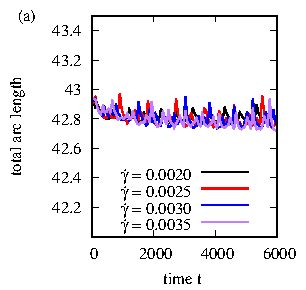
\includegraphics[height=2in]{ArcLength.pdf}
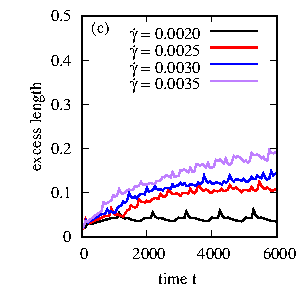
\includegraphics[height=2in]{ExcLength.pdf}
\end{center} 
  \caption{(a) Total arc lengths of the midplanes over time in different shear rates; (b) From exponential fits in panel (a), we obtain the decay rate for a number of different shear rates;
  (c) Reduced area transitions over time. (d) Excess length of the midplanes.
A set of shear rates $\dot\gamma=\{0.002,0.0025,0.003,0.0035\}$ is used in simulations. 
A slower shear rate generates a faster convergence in the reduced area and smaller excess length. 
  }
    \label{figure4}
\end{figure}


\todo[inline]{Figure/Table of the friction coefficient for different shear rates (needs to revise)}


The intermonolayer friction coefficient of the Janus-vesicle is calculated from the ratio of friction force and the 
slip velocity. This quantity is given by 
\begin{equation}
b = \frac{F_f}{v^\parallel} = \frac{F_f}{\int_{\Sigma_M} R \dot\theta dS}.
\end{equation}
%
where $v^\parallel$ represents the tangential velocity at the midplane and $\Sigma_M$ the curve determined by the midplane.


\begin{figure}
\begin{center}
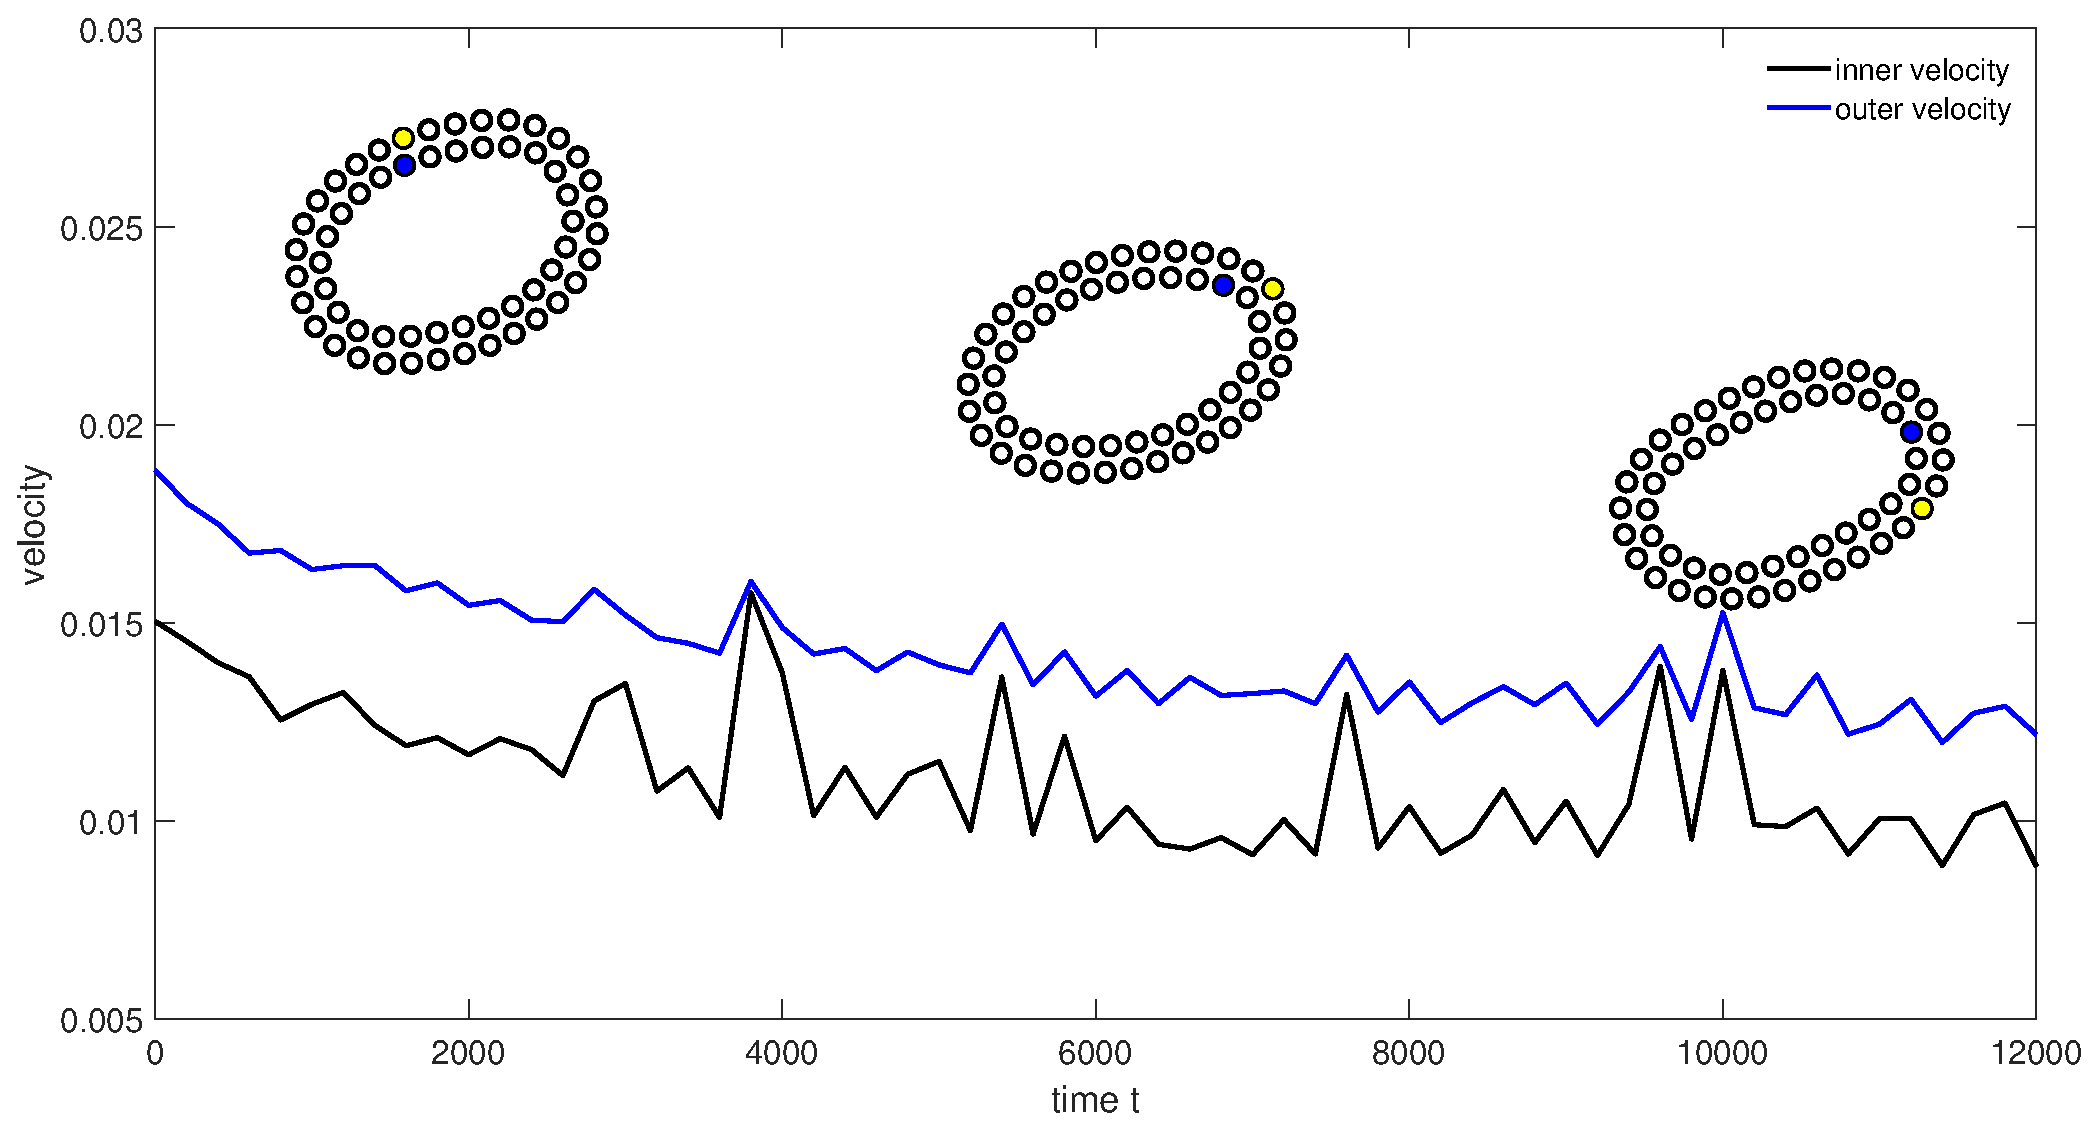
\includegraphics[width=0.8\textwidth]{Slip.eps}
\end{center} 
  \caption{The schematic of the intermonolayer slip over a period of time. Taking shear rate $\dot\gamma=0.005$ as an example, we denote the mean angle between each particle pair $\theta(t)$ where the angle is calculated from the relative position of particles using the vesicle center of mass position. The configuration plots have two fixed particles marked in yellow and blue and labeled with the corresponding time $t=\{2000,5200,9000\}$. The midplane curve is denoted as $\Sigma_M$.
  }
    \label{figure5}
\end{figure}


\begin{table}
\caption{Friction Coefficients}
\centering    
\begin{tabular}{c c c c c c c c }
\hline                    
$\dot\gamma$ & 0.0020 & 0.0025 & 0.0030 & 0.0035 & 0.0040 & 0.0045 & 0.0050\\
\hline 
$F_{f}$ &  &  &  &  &  &  &   \\[1ex]
$\dot\theta$             &  &  &  &  &  &  & \\ [1ex]
$b$             &  &  &  &  &  &  & \\ 
\hline    
\end{tabular} 
\label{table1}
\end{table}


\subsubsection{Vesicle in a Parabolic Flow}

The background flow for this set of simulations is given by

\begin{equation}
{\bf v}_\infty = v_{max}\left[ 1 - \left( \frac{y}{wR_0}\right)^2 \right]{\bf e}_x,
\end{equation}
%
where $v_{max}$ is the flow strength and $w$ controls the shape of the flow. $R_0$ is defined as the radius of the initial vesicle midplane. Figure~\ref{figure6} gives a final configuration for one specific case where the circular vesicle is initially placed above the $x$-axis.


\begin{figure}
\centering
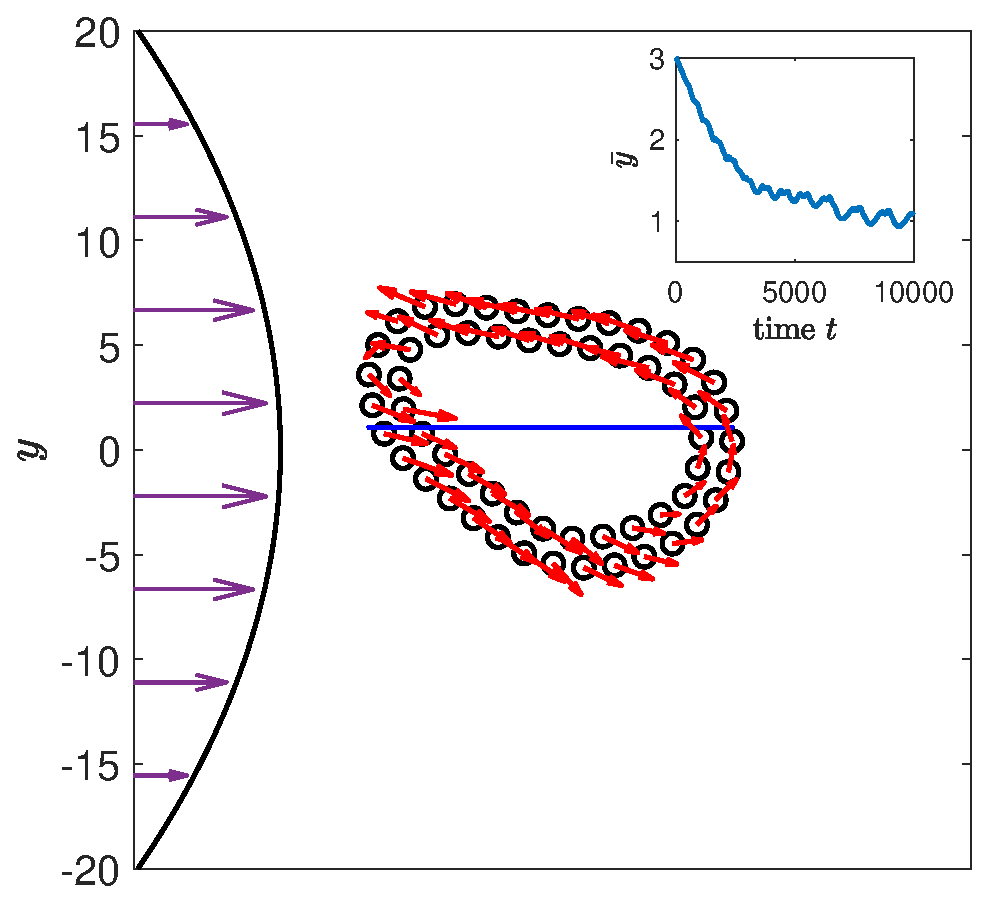
\includegraphics[height=2in]{parabolic.eps}
  \caption{Vesicle under a parabolic flow where the strength of the flow $v_{max}=8.0$ and the control parameter $w=10$. The configuration is the state when $t=10000$.
  }
    \label{figure6}
\end{figure}


\subsubsection{Membrane Ruptures}


With the choice of a large shear rate, a pore formation or a complete membrane rupture can be observed during simulations. Figure~\ref{figure7} shows a demonstration of a vesicle under a shear flow with shear rate $\dot\gamma=0.1$. An interesting phenomenon occurs in panels (c) and (d) where two separated bilayers move along the background shear flow symmetrically. Consequently, a periodic motion for bilayers may occur 
with the choices of shear rates. One can expect that these two layers will flow far apart from each other for much higher shear rates.



\begin{figure}
\centering
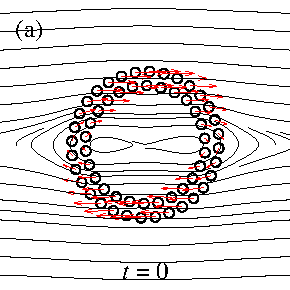
\includegraphics[height=2in]{N58_rupt_0.pdf}
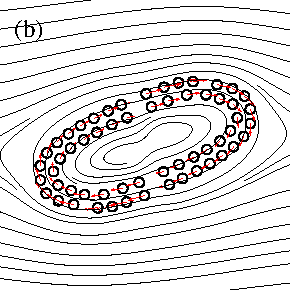
\includegraphics[height=2in]{N58_rupt_200.pdf}
\\
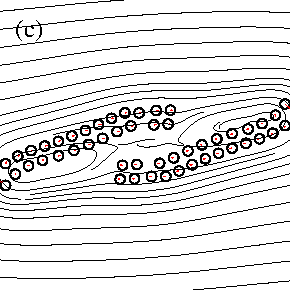
\includegraphics[height=2in]{N58_rupt_400.pdf}
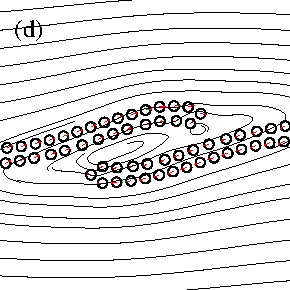
\includegraphics[height=2in]{N58_rupt_600.pdf}
  \caption{Membrane rupture occurs when the shear rate is beyond a certain threshold. Here the shear rate is $\dot\gamma = 0.1$. Starting with a circular shape (panel (a)), the vesicle is stretched by the background flow and multiple pores appear (panel (b)). (c)-(d) are the later states during the simulation.
  }
    \label{figure7}
\end{figure}


%


\subsection{Two Vesicles in a Linear Flow}


\begin{figure}
\centering
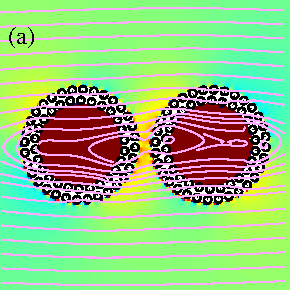
\includegraphics[height=2in]{N116_shear_0.pdf}
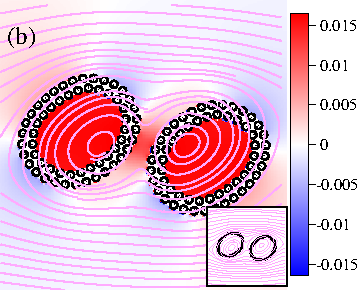
\includegraphics[height=2in]{N116_shear_2500.pdf}\\
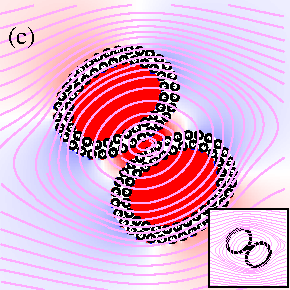
\includegraphics[height=2in]{N116_shear_5000.pdf}
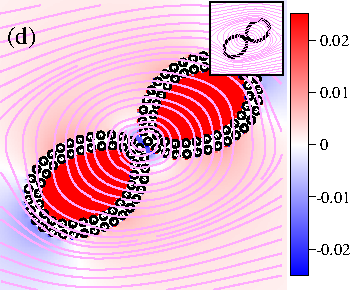
\includegraphics[height=2in]{N116_shear_7500.pdf}
  \caption{Two vesicles under a shear flow where the dimensioneless shear rate is $\dot\gamma=0.005$; The initial configuration is shown in panel (a). The background color indicates the magnitude of fluid pressure. From dark red to dark blue, it represents the the pressure varies from high to low values. The color bar is valid for all panels. Streamlines are plotted in purple. The insets of all panels are generated from the results of continuum modeling simulations and the streamlines have a perfect agreement to the numerical results.
  }
    \label{figure9}
\end{figure}



\subsubsection{Shear Flow}
Two vesicles in a shear flow is presented in Figures~\ref{figure9} where centers of mass are placed on the same horizontal level. With the same starting state as one in the extensional flow, panels (b)-(d) in Figure~\ref{figure8} are the observed phenomena when two vesicles are in a shear flow where the flow is given by $\dot x = \dot\gamma y$. 
An interesting event occurs in the simulation that a rotational behavior with an adhesive effect can be observed and tuned. In other words, the adhesive behavior will be absent when two vesicles are centered 
at a different level and are well separated in $y$-direction.

%\todo[inline]{Migration pattern and/or separation distance. See Fig 8 in
%JCP paper by Rahimian, Veerapaneni, and Biros.}



\begin{figure}
\centering
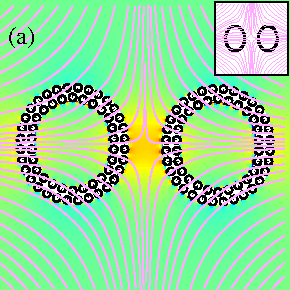
\includegraphics[height=2in]{N116_ext_0.pdf}
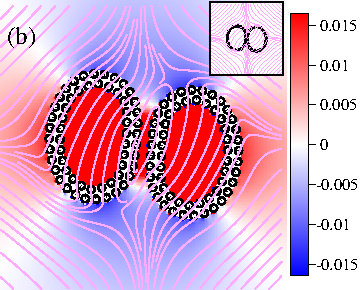
\includegraphics[height=2in]{N116_ext_2000.pdf}\\
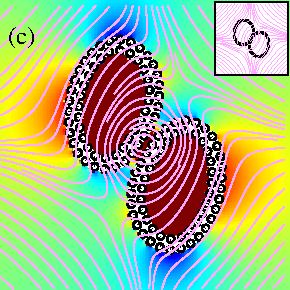
\includegraphics[height=2in]{N116_ext_4000.pdf}
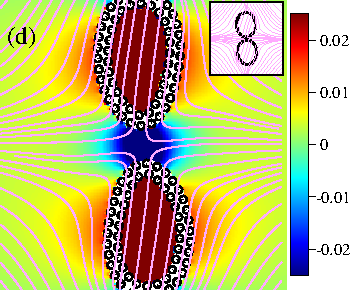
\includegraphics[height=2in]{N116_ext_6500.pdf}
  \caption{Two vesicles under an extensional flow where the dimensioneless shear rate is $\dot\gamma=0.005$; The initial configuration is shown in panel (a). The background color indicates the magnitude of fluid pressure. From dark red to dark blue, it represents the the pressure varies from high to low values. The color bar is valid for all panels. Streamlines are plotted in purple. The insets show the results produced from using continuum model that the streamlines have perfect agreements with the present results.
  }
    \label{figure8}
\end{figure}


\subsubsection{Extensional Flow}

Figures~\ref{figure8} show the numerical results of simulations when two vesicles are in an extensional flow. Starting from the initial configuration (shown in panel (a)), panels (b)-(d) show the transitions of two vesicles moving under an extensional flow. The extensional flow is stretching along the $y$ direction and squeezing in $x$ direction with shear rate $\dot\gamma=0.005$. Since two bilayers are close enough
from the beginning of the run, two vesicles are first pushed toward each other then separate along the streamline. The short range repulsion plays an important role to avoid structure collisions and 
this result can be compared with some findings in continuum modeling simulations.
The pressure plots in Figure~\ref{figure8} provide a realistic result where the pressure is much higher in the gap between two nearby vesicles.

%may need to add more here


\todo[inline]{Make figure of the paths of the two centroids....}



\section{\label{conclusion}Conclusion}


\begin{acknowledgments}
%We would like to acknowledge 
\end{acknowledgments}

\appendix

\section{Appendices}
\label{sec:appendixA}
The stress ${\bf T}$ contains the gradient of the double layer
potential. This introduces an inherent difficulty in evaluating stress
on the boundary.  To overcome the difficulty of evaluation on
$\Sigma_p$, for instance, we decompose $u$ into singular and nonsingular
parts:
\begin{equation}
u = u_p + v_p
\end{equation}
where  
\begin{equation}
u_p(x) = \int_{\Sigma_p} \frac{\partial G(x,y)}{\partial \nnu} \eta(y) \,\dif S(y).
\end{equation}
It turns out that the contribution to the force and torque coming from the singular
part vanishes. In particular, we will prove the identity
\begin{equation}
\label{eq:recipforcetorque}
F_p + iG_p= \int_{\Sigma_p} \gamma ({\bf I}+i{\bf X})J_{p} \,\dif S
\end{equation}
where
 \begin{equation}
\label{eq:jumpstress1}
J_{p} = 2\rho^{-1} \eta  v_p \nnu 
+ 2\rho \nabla \eta \cdot \tau_i(\nabla v_p \cdot \tau_i \nnu -  \nabla
   v_p \cdot \nnu \tau_i).
\end{equation}
Here $\nnu$ is the unit normal, $\{\tau_i\}_{i=1}^2$ are orthonormal tangent vectors,
and ${\bf X}$ is the skew symmetric matrix with axial vector $x$, i.e.
\[X_{ij} = \varepsilon_{ikj}x_k,\quad {\bf X}v = x\times v\]
where $\boldsymbol{\varepsilon}$ is the third-order alternating tensor.
We employ the Einstein summation convention and use complex vectors to streamline the presentation, $i^2 = -1$.

The benefit of using \eqref{eq:recipforcetorque} is that the integrand  is nonsingular.
The density function $\eta$ has the same smoothness as the boundary data
and $v_p$ is real-analytic in a neighborhood of $\Sigma_p$.

To prove \eqref{eq:recipforcetorque}, write
\begin{align*}
  {\bf T}
  &=
  \sigma[u_p,u_p]
  +(\sigma[u_p,v_p]
  +\sigma[v_p,u_p])
  +\sigma[v_p,v_p] \\
  &= {\bf T}_1 + {\bf T}_2 + {\bf T}_3
\end{align*}
where
\[
\sigma[u,v]
= \rho^{-1} uv {\bf I} + \rho \nabla u \cdot \nabla v {\bf I} - 2 \rho \nabla u \otimes \nabla v.
\]
\begin{lemma}
  \label{eq:stress_div_lemma}
  \begin{equation}
    \label{eq:decompdivfree}
    \nabla \cdot {\bf T}_j = 0, \quad
    \nabla \cdot (\xx \times {\bf T}_j) = 0,\quad j = 1, 2, 3.
  \end{equation}
\end{lemma}
\begin{proof}
  Observe that
  \begin{align*}
    (\nabla \cdot {\bf T})_j &=
    \nabla_k   T_{jk} \\
    &= \rho^{-1} 2u \nabla_j u + \rho(2\nabla_{kl}^2 u \nabla_l u  - 2 \nabla_{kj}^2 u \nabla_k u
    - 2 \nabla_j u \nabla_{kk}^2 u )\\
    &=2\rho^{-1}(-\rho^2 \Delta u + u)\nabla_k u .
  \end{align*}
  Since $-\rho^2 \Delta u + u = 0$, we have $\nabla \cdot {\bf T} = 0$.
  Furthermore,
  \begin{align*}
    (\nabla \cdot (x\times {\bf T} ))_j
    &= (\nabla \cdot ({\bf X} {\bf T} ))_j
    = \nabla_k (X_{jl} T_{lk})
    = \nabla_k (\epsilon_{jml}x_m T_{lk})\\
    &= \varepsilon_{jml} T_{lm} + \varepsilon_{jml}x_m \nabla_k T_{lk}\\
    &= (\boldsymbol{\varepsilon}:{\bf T} + {\bf x} \times \nabla \cdot {\bf T})_j.
  \end{align*}
  Since ${\bf T}$ is symmetric $\boldsymbol{\varepsilon}:{\bf T} = {\bf 0}$, and we get
  $\nabla \cdot (x \times {\bf T}) = 0$ as well.

  The functions $u_p$ and $v_p$ also solve the equation $-\rho^2 \Delta u + u = 0$.  Thus
  \eqref{eq:decompdivfree} holds for $j = 1, 3$. Finally,
  \eqref{eq:decompdivfree} holds for $j = 2$ because
  ${\bf T}_2 = {\bf T} - {\bf T}_1 - {\bf T}_3$.
\end{proof}


Using Lemma \ref{eq:stress_div_lemma}, we will establish that
\begin{equation}
  \label{eq:prejump}
  F_p + i G_p = \gamma \int_{\Sigma_p}  ({\bf U}_2\nnu)^+ - ({\bf
  U}_2\nnu)^-\,\dif S
\end{equation}
where ${\bf U}_j = ({\bf I} + i {\bf X}){\bf T}_j$ for $j = 1, 2, 3.$
The stress ${\bf U}_2$ has a jump discontinuity at $\Sigma_p.$
The plus and minus superscripts denote
the limit taken along points in $U_p^c$ and along points in $U_p$
respectively.
${\bf U}_1$ and ${\bf U}_3$ are real-analytic in a neighborhood of $\overline{U_p}$
and have no jump-discontinuity at $\Sigma_p$.
To derive \eqref{eq:prejump}, we expand
\begin{align*}
  F_p + i G_p
  &= \gamma \int_{\Sigma_p} {\bf T} \nnu + ix \times {\bf T} \nnu \,\dif S \\
  &= \gamma \int_{\Sigma_p}  {\bf U}_1\nnu  + ({\bf U}_2\nnu)^+ + {\bf
  U}_3\nnu\,\dif S
\end{align*}
The function $u_p$ is real-analytic and
$\nabla \cdot {\bf U}_1 = 0$ throughout $\mathbb{R}^n \setminus U_p$.
By the divergence theorem, we get
\begin{equation*}
  \int_{\Sigma_p}  {\bf U}_1 \nnu\,\dif S
  = \int_{\mathbb{R}^n \setminus U_p} \nabla \cdot {\bf U}_1 \,dx = 0.
\end{equation*}
Next, $v_p$ is real-analytic and
$\nabla \cdot {\bf U}_3 = 0$ in $U_p$. Therefore
\begin{equation*}
  \int_{\Sigma_p}  {\bf U}_3 \nnu\,\dif S
  = -\int_{U_p} \nabla \cdot {\bf U}_3 \,dx = 0.
\end{equation*}
Finally, $\nabla \cdot {\bf U}_2= 0$ in $U_p$. This gives
\[
0 = -\int_{U_p} \nabla \cdot {\bf U}_2 \,dx = \int_{\Sigma_p}  ({\bf
U}_2 \nnu)^-\,\dif S.
\]
Combining the last four equations give \eqref{eq:prejump}.

\begin{proof}[Proof of \eqref{eq:recipforcetorque}]
  The main ingredients of the proof are the jump relations
  for $u_p$. For $x_0 \in \Sigma_p$,
  \begin{enumerate}
  \item $ \lim_{x \to x_0^\pm } u_p(x) = \pm\frac{1}{2}\eta(x_0) + (D\eta)(x_0)$
  \item $ \lim_{x \to x_0^+ } (\nabla u_p \cdot \nnu) (x) = \lim_{x \to
    x_0^-} (\nabla u \cdot \nnu)(x)$
  \end{enumerate}
  Furthermore,
  combining (i) and (ii) gives
  \begin{align*}
    \nabla u_p^+ - \nabla u_p^-
    &= \nabla (u_p^+ - u_p^-) \cdot t_i t_i +  (\nabla  u_p^+\cdot
    \nnu  - \nabla u_p^- \cdot \nnu) \nnu\\
    &= \nabla \eta \cdot \tau_i \tau_i
  \end{align*}
  where $\{\tau_i\}_{i=1}^n$ are an orthonormal tangent vectors.
  We can use these relationships to derive an expression for the jump in
  normal stress.
  \begin{align*}
    &({\bf T}_2\nnu)^+ - ({\bf T}_2\nnu)^-
    \\
    &= 2\rho^{-1} u_p^+v_p \nnu + 2\rho \nabla u_p^+ \cdot \nabla v_p
    \nnu
    - 2 \rho \nabla u_p^+  \nabla v_p \cdot \nnu
    - 2 \rho \nabla v_p  \nabla u_p^+ \cdot \nnu\\
    &-2\rho^{-1} u_p^-v_p \nnu - 2\rho \nabla u_p^- \cdot \nabla v_p \nnu
    + 2 \rho \nabla u_p^-  \nabla v_p \cdot \nnu
    + 2 \rho \nabla v_p  \nabla u_p^- \cdot \nnu\\
    &= 2\rho^{-1} \eta v_p \nnu + 2\rho \nabla \eta \cdot \tau_i \tau_i
    \cdot \nabla v_p \nnu
    - 2\rho \nabla \eta \cdot \tau_i \tau_i \nabla v_p \cdot \nnu + 0\\
    &= J_p.
  \end{align*}

  Applying the above relations to the integrand of \eqref{eq:prejump} yields
  \[
  ({\bf U}_2\nnu)^+ - ({\bf U}_2\nnu)^-
  =
  ({\bf I} + i {\bf X})(({\bf T}_2\nnu)^+ - ({\bf T}_2\nnu)^-)
  = ({\bf I} + i {\bf X})J_p
  \]
  This completes the proof of \eqref{eq:recipforcetorque}.
\end{proof}




%\section{\label{A2} Comparison between Continuum Model and the Proposed Model}
%
%\begin{figure}
%\centering
%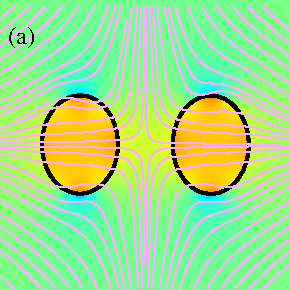
\includegraphics[height=1.2in]{N116_cont_a.pdf}
%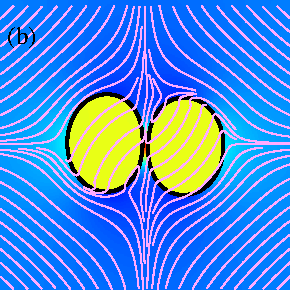
\includegraphics[height=1.2in]{N116_cont_b.pdf}
%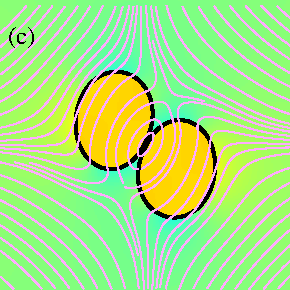
\includegraphics[height=1.2in]{N116_cont_c.pdf}
%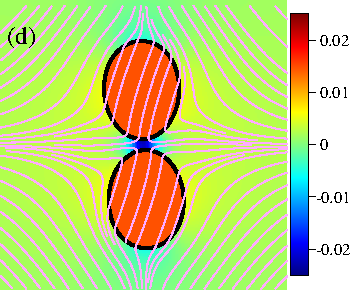
\includegraphics[height=1.2in]{N116_cont_d.pdf}
%  \caption{Two vesicles under an extensional flow where the dimensioneless shear rate is $\dot\gamma=0.005$; Continuum modeling.....
%  }
%    \label{figureB}
%\end{figure}










\bibliographystyle{jfm}
\bibliography{reference}% Produces the bibliography via BibTeX.





%\bibliographystyle{jfm}
%\bibliography{jfm}
%Use of the above commands will create a bibliography using the .bib file. Shown below is a bibliography built from individual items.


%\bibliography{jfm2esam}

%\begin{thebibliography}{99}
%
%\expandafter\ifx\csname natexlab\endcsname\relax
%\def\natexlab#1{#1}\fi
%\expandafter\ifx\csname selectlanguage\endcsname\relax
%\def\selectlanguage#1{\relax}\fi
%
%\bibitem[Batchelor (1971)]{Batchelor59}
%{\sc Batchelor, G.K.} 1971 {Small-scale variation of convected quantities like temperature in turbulent fluid part1, general discussion and the case of small conductivity}, {\it J. Fluid Mech.}, {\bf 5}, pp. 3-113-133.
%
%\bibitem [Bouguet (2008)]{Bouguet01}
%{\sc Bouguet, J.-Y} 2008 Camera Calibration Toolbox for Matlab {\url{http://www.vision.caltech.edu/bouguetj/calib_doc/}}.
%
% \bibitem[Briukhanovetal et al (1967)] {Briukhanovetal1967}
%{\sc Briukhanov, A. V.,   Grigorian, S. S., Miagkov,  S. M., Plam, M. Y.,   I. E. Shurova, I. E.,   Eglit, M. E. and Yakimov, Y. L.} 1967
%{On some new approaches to the dynamics of snow avalanches},
%{\it Physics of Snow and Ice,  Proceedings of the International Conference on Low Temperature Science}
%{Vol 1} pp. 1221--1241 {Institute of Low Temperature Science, Hokkaido University, Sapporo, Hokkaido, Japan}.
%
%\bibitem[Brownell (2004)]{Brownell04}
% {\sc Brownell,  C.J.  and Su,  L.K.} 2004  {Planar measurements of differential diffusion in turbulent jets}, {\it AIAA Paper},  pp. 2004-2335.
%
%\bibitem[Brownell and Su (2007)] {Brownell07}
%  {\sc Brownell, C.J. and  Su, L.K.} 2007 {Scale relations and spatial spectra in a differentially diffusing jet}, {\it AIAA Paper}, pp 2007-1314.
%
%\bibitem [Dennis (1985)] {Dennis85}
% {\sc  Dennis, S.C.R.} 1985 {Compact explicit finite difference approximations to the Navier--Stokes equation},  { In \it Ninth Intl Conf. on Numerical Methods in Fluid Dynamics},  {ed Soubbaramayer and J.P. Boujot},  {Vol 218}, {\it Lecture Notes in Physics}, pp. 23-51. Springer.
%
%\bibitem [Edwards et al. (2017)]{EdwardsVirouletKokelaarGray2017}
%{\sc Edwards, A. N., Viroulet, S., Kokelaar, B. P. and Gray, J. M. N. T.} 2017 Formation of levees, troughs and elevated channels by avalanches on erodible slopes {\it J. Fluid Mech.}, {\bf 823}, pp. 278-315.
%
%\bibitem[Hwang et al (1970)] {Hwang70}
% {\sc Hwang,  L.-S.  and  Tuck, E.O.} 1970 On the oscillations of harbours of arbitrary shape {\it J.~Fluid Mech.}, {\bf42}, pp 447-464.
%
%\bibitem[Josep and Saut (1990)] {JosephSaut1990}
% {\sc Joseph, Daniel D. and Saut, Jean Claude} 1990 Short-wave instabilities and ill-posed initial-value problems {\it Theoretical and Computational Fluid Dynamics}, {\bf 1},  pp.191--227,  {\url{http://dx.doi.org/10.1007/BF00418002}}.
%
%\bibitem[Worster (1992)] {Worster92}
%{ \sc  Worster, M.G.} 1992 The dynamics of mushy layers {\it Interactive dynamics of convection and solidification},
%{(ed. S.H. Davis and H.E. Huppert and W. Muller and M.G. Worster)}, pp. 113--138 {Kluwer}.
%
%\bibitem[Koch(1983)] {Koch83}
%{\sc Koch, W.} 1983 Resonant acoustic frequencies of flat plate cascades {\it J.~Sound Vib.}, {\bf 88}, pp. 233-242.
%
%\bibitem[Lee(1971)] {Lee71}
%{\sc Lee,  J.-J.}  1971 Wave-induced oscillations in harbours of arbitrary geometry {\it J.~Fluid Mech.}, {\bf 45}, pp. 375-394.
%
%\bibitem[Linton and  Evans (1992)] {Linton92}
% {\sc  Linton, C.M. and  Evans, D.V.} 1992 The radiation and scattering of surface waves by a vertical circular cylinder in a channel {\it Phil.\ Trans.\ R. Soc.\ Lond.}, {\bf 338}, pp. 325-357.
%
%\bibitem [Martin(1980] {Martin80}
% {\sc  Martin, P.A.} 1980 On the null-field equations for the exterior problems of acoustics {\it Q.~J. Mech.\ Appl.\ Maths},{\bf 33}, pp. 385--396.
%
%\bibitem [Rogallo(1981)] {Rogallo81}
% {\sc Rogallo,  R.S.} 1981 Numerical experiments in homogeneous turbulence  { {\it Tech. Rep.} 81835}  {NASA Tech.\ Mem}.
%
%\bibitem[Ursell(1950)] {Ursell50}
%{\sc  Ursell, F.} 1950 Surface waves on deep water in the presence of a submerged cylinder i {\it Proc.\ Camb.\ Phil.\ Soc.}, {\bf 46}, pp.141--152.
%
%\bibitem[Wijngaarden (1968)]{Wijngaarden68}
%{\sc van Wijngaarden, L.} 1968 On the oscillations Near and at resonance in open pipes {\it J.~Engng Maths},{\bf 2}, pp. 225--240.
%
%\bibitem[Miller (1991)]{Miller91}
%{ \sc  Miller, P.L.} 1991 Mixing in high Schmidt number turbulent jets {school {PhD thesis}} {California Institute of Technology}.
%
%\end{thebibliography}

%% End of file `jfm2esam.bib'.

\end{document}
